\documentclass[12pt,letter]{article}
% \usepackage[utf8]{inputenc}
\usepackage{graphicx}
\usepackage{amsmath}
\usepackage{amssymb}
\usepackage[left=2cm,right=2cm,top=3cm,bottom=2cm]{geometry}
\usepackage{float}
\usepackage[super,sort&compress,comma]{natbib} \usepackage[font={small}]{caption} %scriptsize = 8pt; footnotesize = 9pt; small = 10pt; normalsize = 11pt (set on line 4 above)
\usepackage[labelfont=bf]{caption}
\usepackage{bm}
\usepackage[T1]{fontenc}
\usepackage[version=4]{mhchem}
\usepackage{textcomp}
\usepackage{titling}
 \newcommand{\textapprox}{\raisebox{0.5ex}{\texttildelow}}
\usepackage{color}
\include{MyCommand}
\newcommand{\JPH}[1]{{\color{red}{#1}}}
\usepackage{tabularx}
\usepackage{bm}
\usepackage[left]{lineno}
\linenumbers


 \setcounter{figure}{0}
 \let\oldthefigure\thefigure
 \renewcommand{\figurename}{Supplementary Figure}

\renewcommand\refname{Supplementary References}

\begin{document}
\title{Supplementary Information: Title}
\author{Joseph Heindel$^{1,2}$, Teresa Head-Gordon$^{1,2,3}$}
\date{\vspace{-10ex}}
\maketitle
\noindent
\begin{center}
$^1$Kenneth S. Pitzer Theory Center and Department of Chemistry\\
$^2$Chemical Sciences Division, Lawrence Berkeley National Laboratory\\
$^3$Departments of Bioengineering and Chemical and Biomolecular Engineering\\
University of California, Berkeley, CA, USA


corresponding author: thg@berkeley.edu
\end{center}

\newpage

In the course of developing this model, we found that we were unable to reproduce the
expected correlation between change in bond length and change in harmonic frequency
for \ce{O-H} stretches.\cite{boyer2019beyond} We ultimately determined that the failure
of our model to reproduce this correlation was due to a lack of coupling between
our bonding potential and the environment. To that end, we extended our morse potential
to be field-dependent in a manner first described elsewhere.\cite{boyer2019beyond} In short,
the field-dependence of the potential requires specifying the first and second dipole
derivatives along the \ce{O-H} stretch.

Rather than treating these as fitting parameters, we computed the dipole derivatives
from electronic structure as follows. First, we scan along an \ce{O-H} stretch
and compute the total dipole moment, $\mu$, at each point along the scan. This dipole
moment is then projected onto the \ce{O-H} bond vector,
$\mu_{\mathrm{OH}}=\frac{R_{\mathrm{OH}}\cdot \mu}{|R_{\mathrm{OH}}|}$. This allows
us to isolate how the dipole changes as the \ce{O-H} vibrates in a particular environment.

We considered three different environments to see how the dipole derivatives depend on the
local environment and ultimately chose a set of parameters we deemed appropriate for
polarization and one to represent the full system. Remember that in EDA, the polarization
energy represents the response of a molecule to the rest of the environment plus mutual
polarization. To that end, we computed an \ce{O-H} stretch of an isolated \ce{H2O} in
a polarizable continuum described by the COSMO model.\cite{klamt2011cosmo} This resulted
in the dipole surface shown with circles in Fig. \ref{fig:dip_derivatives}. The lines
are fits with a second order polynomial,
$\Delta\mu_{\mathrm{OH}}=\mu_{\mathrm{OH}}^{(1)}\Delta R_{\mathrm{OH}}+\mu_{\mathrm{OH}}^{(2)}\Delta R_{\mathrm{OH}}^2$.
For \ce{H_2O} in a dielectric, we find $\mu_{\mathrm{OH}}^{(1)}=0.345$ and $\mu_{\mathrm{OH}}^{(2)}=0.095$. This
is to be compared to the same values for an isolated \ce{H2O} of $\mu_{\mathrm{OH}}^{(1)}=0.165$ $\mu_{\mathrm{OH}}^{(2)}=-0.012$.
The effect of an environment is, therefore, to promote dissociation to ionic products rather than
radicals which is what the change in sign of $\mu_{\mathrm{OH}}^{(2)}$ implies and to make it easier
to elongate the \ce{O-H} bond which is what the magnitude of $\mu_{\mathrm{OH}}^{(1)}$ means.

Interestingly, when the environment is represented by an actual molecule, as with \ce{(H_2O)_2},
the second dipole derivative increases by a lot and increases even further when when a dielectric
continuum is used. This is seen in the points marked with squares in Fig. \ref{fig:dip_derivatives}.
We attribute this large non-linearity in the dipole surface to the role of charge delocalization,
which makes these parameters suitable for the full potential which includes charge transfer.

A water dimer, however, is not a representative environment for liquid water, or even large
water clusters. To remedy this, we constructed a tetrahedrally coordinated water dimer, \ce{(H2O)_{2+6}}.
The notation \ce{(H2O)_{2+6}} indicates that this is a water dimer solvated by six other water
molecules. The cartesian coordinates are available with the manuscript. When this larger solvation environment
is used, we see a further increase in the dipole derivatives beyond just a water dimer.
The dipole derivatives for the central \ce{O-H} stretch in \ce{(H2O)_{2+6}} are $\mu_{\mathrm{OH}}^{(1)}=1.082$ and
$\mu_{\mathrm{OH}}^{(2)}=1.54$. When these values are used in the model, the
$\Delta\omega$ vs $\Delta R_e$ slope is $\approx -17.1\ \mathrm{cm^{-1}/.001\AA}$ over the same clusters.

 \begin{figure} [H]
    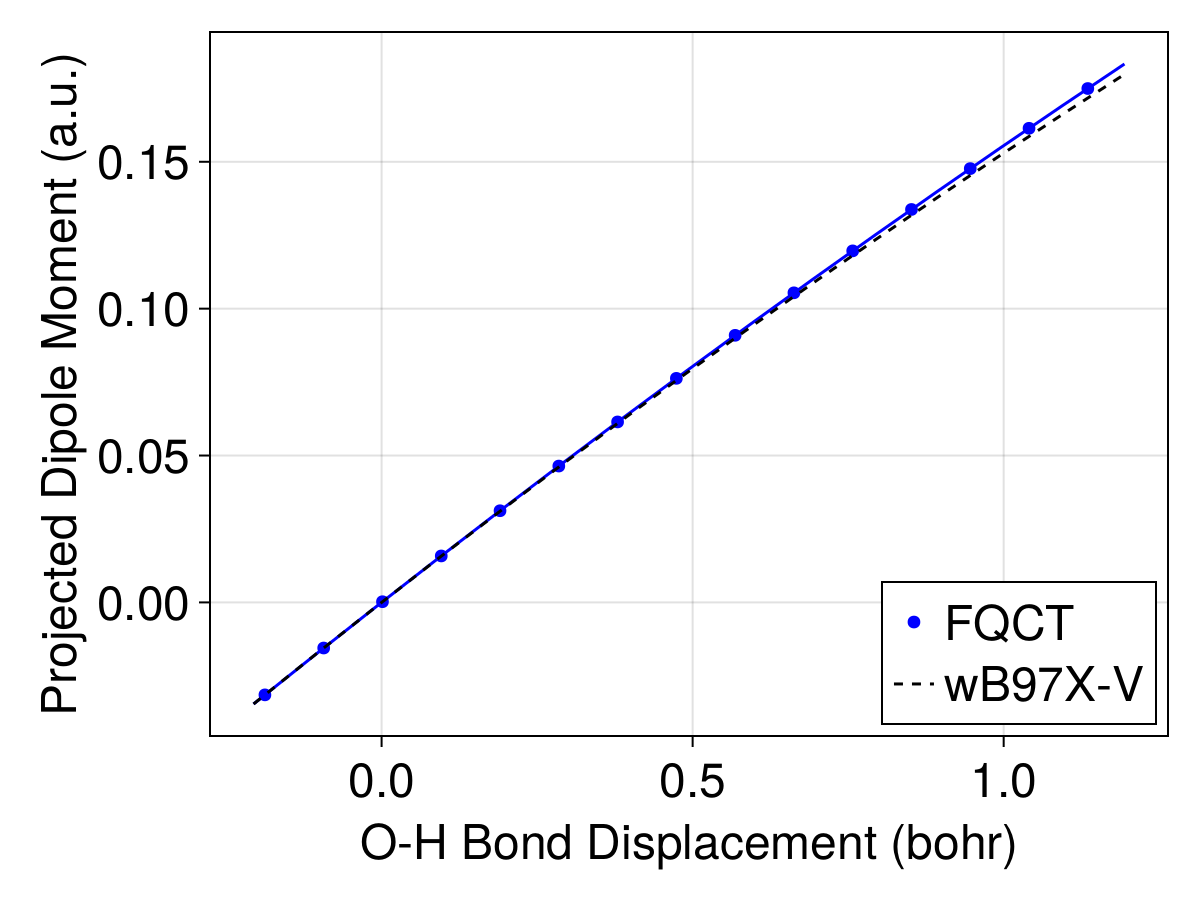
\includegraphics[width=\textwidth]{figures/dipole_derivatives.png}
    \caption{\textit{Projected dipole moments along various O-H stretches.}
    The dipole moment of \ce{(H2O)}, \ce{(H2O)_2}, and \ce{(H2O)_{2+6}} are computed with
    $\omega$B97X-V/def2-QZVPPD as a function of the \ce{O-H} stretch distance. All other degrees of freedom are fixed.
    The dipole moment is projected along the \ce{O-H} stretch unit vector. \ce{(H2O)_{2+6}}
    is a water dimer with six additional water molecules placed so that the water dimer is
    tetrahedrally coordinated. The blue points and lines are gas-phase systems while the
    red points and lines include a polarizable continuum. Each point is connected vertically
    to make it clear they are the same structure but in the presence of a polarizable continuum.
    Circles are used for a single water molecule, squares for a water dimer, and triangles for
    the tetrahedrally solvated water dimer. See text for more details and values of computed dipole derivatives.
}
    \label{fig:dip_derivatives}
\end{figure}

In principle, the curves in Figure \ref{fig:dip_derivatives} should eventually be equal when sufficient
explicit solvent is included in the calculation. Since the dipole derivatives computed from
\ce{(H2O)_{2+6}} are not sufficient to reproduce the Badger correlation, we increase
the dipole derivatives until the appropriate correlation is reproduced. This results in values
of $\mu_{\mathrm{OH}}^{(1)}=1.19$ and $\mu_{\mathrm{OH}}^{(2)}=3.69$. To be completely rigorous,
these dipole derivatives should be functions of the local environment, but we have not explored
that possibility in this work since choosing them to be constants works quite well.

\bibliographystyle{unsrtnat}
\bibliography{references}
    
\end{document}
